\chapter {Interfejs SWD i programator}

Do komunikacji komputerów klasy PC poprzez interfejs SWD (Serial Wire Debug) używa się programatorów podpinanych do komputera przez port USB. Najpopularniejszy na rynku standard wyprowadzeń do obsługi urządzeń z rodziny ARM Cortex-M to ARM JTAG 20, posługujący się dwurzędowym wtykiem 2x10 pinów. Multiplekser SWD został stworzony do współpracy z takimi właśnie programatorami. Na potrzeby testów użyty został programator J-Link EDU. Jest to jeden z najpopularniejszych i tańszych programatorów, który posiada bardzo dobre wsparcie producenta, mogąc działać pod kontrolą systemów operacyjnych Windows, Linux i Mac OS.

\section{Serial Wire Debug}
 $SWD$, czyli Serial Wire Debug to standard interfejsu używany do komunikacji programatora z modułem $DAP$ (Debug Acces Protocol) w urządzeniach z rodziny ARM Cortex-M. Ponadro $SWD$ wymaga mniej wyprowadzeń niż konkurencyjny JTAG.\\
 Wykorzystuje on 2 linie transmisyjne:
 \begin{enumerate}
     \item $SWDIO$ - Dwukierunkowy sygnał danych.  
     \item $SWCLK$ - Sygnał zegara generowany przez sondę debugującą.
 \end{enumerate}
 Ponadto celem rozszerzenia funkcjonalności często używa się z nim linii:
 \begin{enumerate}
     \item $Reset$ -  sygnał reset, zwyczajowo aktywowany niskim stanem
     \item $SWO$ - Serial Wire Output - dedykowany do użycia jako asynchroniczne szeregowe standardowe wyjście. 
     \item $VTref$ - napięcie stanu wysokiego dla wyprowadzeń $SWD$
 \end{enumerate}
 
 \section{Programator J-Link EDU}
  Programator (inaczej sonda debugująca) J-Link EDU (rysunek \ref{J_Link_photo}) posiada interfejsy SWD, JTAG, SPI oraz UART. Wszystkie one mają bufory wejściowe i wyjściowe dopasowujące się do napięcia, jakim posługuje się urządzenie docelowe, przy czym napięcie dla stanu wysokiego musi się zawierać w przedziale od 1.2 V do 5 V a napięcie stanu niskiego to 0 V.
  Ponadto J-Link EDU od wersji V9 wspiera tzw. wirtualny port COM (VCOM), czyli port szeregowy UART w miejscu pinów 5 (Tx) oraz 17 (Rx). (schemat wyprowadzeń znajduje się na rysunku \ref{J_Link_SWD_pinout})
  Na pinie 5V-Supply można dodatkowo włączyć zasilanie 5 V, które może być użyte np. do zasilania urządzenia docelowego. Układ dodatkowo umożliwia pomiar prądu pobranego z tego wyprowadzenia.
  
\begin{figure}[H]
\centering
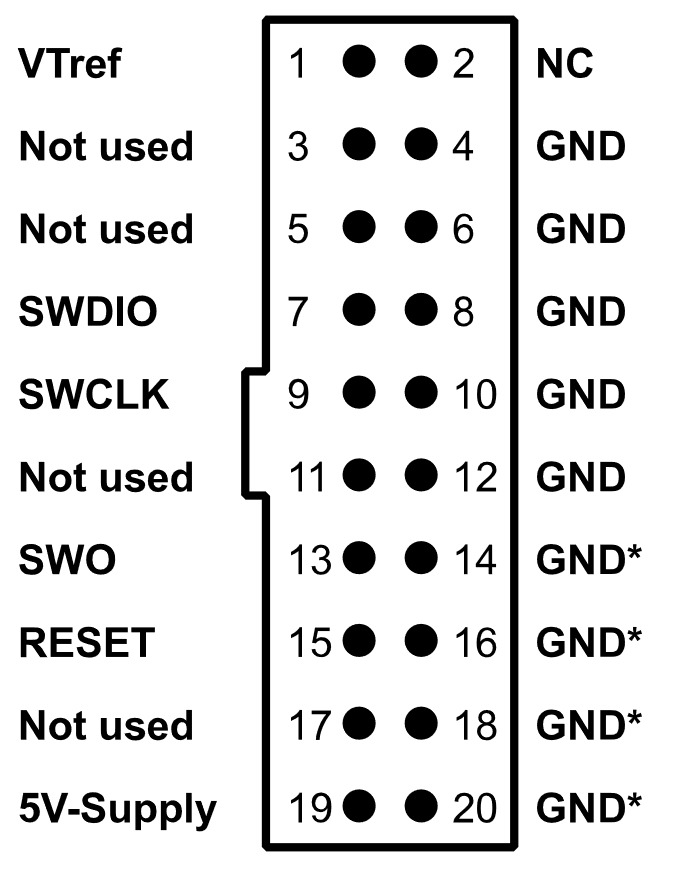
\includegraphics[width=0.35\paperwidth]{images/J-Link_pinout_SWD.png}
\caption{Schemat wyprowadzeń programatora J-Link EDU działającego w trybie SWD. Źródło:\cite{J-Link_pinout_SWD}}
\label{J_Link_SWD_pinout}
\end{figure}

   \begin{figure}[H]
    \centering
    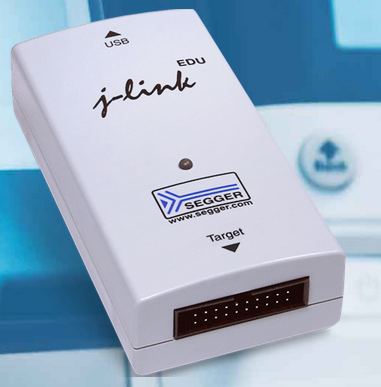
\includegraphics[width=0.45\paperwidth]{images/J-Link_EDU.png}
    \caption{Programator J-Link EDU Źródło:\cite{J-Link_EDU_photo}}
    \label{J_Link_photo}
\end{figure}

  


 


